\documentclass[12pt]{mwrep}
\usepackage{polski}
\usepackage[utf8]{inputenc}
\usepackage[T1]{fontenc}
\usepackage{times}



%\usepackage[margin=20mm, left=30mm]{geometry}

%\usepackage{newtxtext}
%\usepackage{newtxmath}
\usepackage{amsfonts}
\usepackage{amsmath}
\usepackage{bm}
\usepackage{mathtools}
\mathtoolsset{showonlyrefs}


\usepackage{tabularx}
\usepackage{array}
\newcolumntype{Y}{>{\centering\arraybackslash}X}
\newcolumntype{Z}{>{\centering\arraybackslash}p}
\usepackage{multirow}
\usepackage{hyperref}

\usepackage{enumitem}
\usepackage{float}


\usepackage{graphicx}
\usepackage{rotating}
\usepackage{subcaption}


\usepackage{animate}

\renewcommand{\thesection}{\arabic{section}}
\renewcommand{\thesubsection}{\arabic{section}.\arabic{subsection}}
\usepackage{wrapfig}


\begin{document}
	
	\begin{center}
		{\Large\textbf{Symulacje komputerowe}}
	\end{center}
	\begin{center}
		Raport 2
	\end{center}
	
	\noindent Temat: \ \textbf{\boldmath$\alpha$-stabilny proces L\'evy'ego}\\
	Imię i Nazwisko prowadzącego kurs: \ \textbf{Dr Michał Balcerek}	\newline\newline
	

	
	\noindent\begin{tabularx}{\textwidth}{|X |X|}
		\hline
		\begin{center}
			Imię i Nazwisko,\\nr indeksu
		\end{center} &  \begin{center}
			Kacper Budnik\\262286
		\end{center}\\\hline
		Wydział: & Wydział matematyki, W13 \\\hline
		Termin zajęć: & Wtorek,\vphantom{ $11^{1^{5}}$} $11^{15}$\\\hline
		Kod grupy ćwiczeniowej: & T00-70d \\\hline
		Data oddania raportu: & \today \\\hline
		\textbf{Ocena końcowa} &\\\hline
	\end{tabularx}\newline\newline


	\noindent\textbf{Adnotacje i uwagi:}
	
	\newpage
	

	\section{Wstęp}
	\noindent Celem tego raportu jest oszacowanie średniego czasu wyjścia $\alpha$-stabilnego procesu L\'evy'ego z zadanego przedziału w zależności od punktu początkowego. Dodatkowo oszacowane zostało prawdopodobieństwo wyjścia przez dany koniec odcinka. Na koniec, przy pomocy pakietów matematycznych, dopasowaliśmy do oszacowanych wartości funkcję w zależności od punktu startowego $x$ oraz parametru $\alpha$.


	\section{$\alpha$-stabilny proces L\'evy'ego}
	\noindent Procesem L\'evy'ego nazywamy proces $\{X_t: t\geq 0\}$, który spełnia następujące własności\textsuperscript{\cite{Levy_def}}
	\begin{enumerate}[label=\textbf{(\roman*)}, leftmargin=10mm]
		\item trajektorie $X_t$ są $\mathbb{P}$- prawie na pewno prawostronnie ciągłe z lewostronnymi granicami,
		\item $\mathbb{P}\left(X_0=0\right)=1$,
		\item $X_t$ ma niezależna przyrosty,
		\item $X_t$ ma stacjonarne przyrosty.
	\end{enumerate}
	W raporcie tym będziemy badali czas wyjścia procesu L\'evy'ego $X_t^x=X_t+x$, takiego, że 
	\begin{equation}\label{X_dist}
		X_t\sim S_\alpha(t^{1/\alpha},0,0),
	\end{equation}
	z zadanego przedziału $[a, b]$. Zdefiniujmy zmienną
	\begin{equation}\label{eq:tau}
		\tau^x=\inf\left\{t\geq0: X_t^x\notin[a,b]\right\},
	\end{equation}
	oznaczającą wyżej wspomniany czas wyjścia w zależności od punktu startowego.
	Łatwo można pokazać, że $X^{x+y}_t\in[a ,b] \iff X^x_t\in[a-y, b-y]$. Dodatkowo, ponieważ $X_t$ ma rozkład zadany \eqref{X_dist}, to dla $a>0$ zachodzi
	\begin{equation}
		X_{at} \overset{d}{=} S_\alpha\left(\left(at\right)^{1/\alpha},0,0\right)\overset{d}{=}a^{1/\alpha}S_\alpha\left(t^{1/\alpha},0,0\right)
		\overset{d}{=}a^{1/\alpha}X_t,
	\end{equation}
	zatem proces $X_t$ jest procesem $1/\alpha$ podobnym. Z tego faktu wynika, że
	\begin{equation}
		X^x_t=X_t+x\overset{d}{=}\Delta X_{t/\Delta^{\alpha}}+x = \Delta\left(X_{t/\Delta^{\alpha}}-\frac{x}{\Delta}\right)=\Delta X^{x/\Delta}_{t/\Delta^\alpha}.
	\end{equation}
	 Korzystając z tych własności możemy przekształcić \eqref{eq:tau} do postaci
	\begin{equation}
		\begin{split}
		\tau^x&\overset{d}{=}\inf\left\{\Delta^\alpha\frac{t}{\Delta^\alpha}\geq0:\Delta X^{x/\Delta}_{t/\Delta^\alpha}\notin[a, b]\right\} 	=\Delta^\alpha\inf\left\{t^*\geq0:X^{x/\Delta}_{t^*}\notin\left[\frac{a}{\Delta},\frac{b}{\Delta}\right]\right\}\\
		&=\Delta^\alpha\inf\left\{t^*\geq0:X^{(x-s)/\Delta}_{t^*}\notin\left[\frac{a-s}{\Delta},\frac{b-s}{\Delta}\right]\right\}.
		\end{split}
	\end{equation}
	Wybierając teraz $\Delta=(b-a)$ oraz $s=a$ otrzymujemy
	\begin{equation}\label{eq:tau_przeskalowane}
		\tau^x\overset{d}{=}(b-a)^\alpha\inf\left\{t\geq0:X^y_t\in[0,1]\right\}=(b-a)^\alpha\,\widetilde\tau^y,
	\end{equation}
	gdzie $\widetilde\tau^y$ jest czasem wyjścia z przedziału $[0, 1]$, jeśli zaczniemy z punktu $y=\frac{x-a}{b-a}$, czyli z punktu dzielącego ten odcinek w stosunku takim samym jak $x$ dzieli odcinek~$[a, b]$.\vspace{1.5mm}\\
	\noindent Dzięki tym przekształceniom widzimy, że $\mathbb{E}\tau^x$ zależy od odległości $x$ od jednego końca przedziału względem drugiego oraz długości rozważanego odcinka. Ponieważ wiemy już jak wpływa ta długość na średni czas wyjścia, będziemy rozważać jedynie przedział $[0, 1]$.
	\section{Generowania trajektorii}	
	\noindent By móc wygenerować trajektorię procesu musimy umieć generować realizację zmiennej $Y\sim S_\alpha(\sigma,\beta,\mu)$. Cały algorytm został przedstawiona w \cite{art}. Na nasze potrzeby wystarczy algorytm generowania $Y\sim S_\alpha(t^{1/\alpha},0,0)$.\\
	
	\noindent\textbf{Algorytm}\\
	Celem jest wygenerowanie wektora $\left[ X_{t_0},X_{t_1},\dots,X_{t_n} \right]$, gdzie
	\begin{equation}
		t_i=ih, \quad\quad i\in[n]=\{0,1,\dots,n\},\quad h=T/n.
	\end{equation}
	W tym celu stosujemy poniższy algorytm.\\
	\begin{itemize}
		\item $\boldsymbol{\alpha\neq 1}$

		\begin{enumerate}
			\item Generuj realizację zmiennych $V_i$ iid. $\mathcal{U}\left(-\frac{\pi}{2},\frac{\pi}{2}\right)$, $i\in[n-1]$.
			\item Generuj realizację zmiennych $W_i$ iid. $\mathcal{E}xp(1)$, $i\in[n-1]$.
			\item $X_{t_0}=0$.
			\item Wstaw
			\begin{equation}
				X_{t_{i+1}}=X_{t_i} + h^{1/\alpha}\frac{\sin(\alpha V_i)}{(\cos V_i)^{1-\alpha}} \left[\frac{\cos\left(\left(1-\alpha\right) V_i\vphantom{\frac{1}{1}}\right)}{W_i}\right]^{(1/\alpha)/\alpha}.
			\end{equation}
		\end{enumerate}
		\item $\boldsymbol{\alpha= 1}$
		\begin{enumerate}
			\item Generuj realizację zmiennych $V_i$ iid. $\mathcal{U}\left(-\frac{\pi}{2},\frac{\pi}{2}\right)$, $i\in[n-1]$.
			\item $X_{t_0}=0$.
			\item Wstaw
			\begin{equation}
				X_{t_{i+1}}=X_{t_i} + h^{1/\alpha}\tan V_i
			\end{equation}
	\end{enumerate}
	\end{itemize}

	\section{Średni czas wyjścia procesu}
		
	\noindent Do oszacowania średniego czasu wyjścia posłużyłem się metodą Monte Carlo. Czas ten zależy od parametru $\alpha$, dlatego na animacji \ref{anim:time} przedstawiłem otrzymane wykresy dla kolejnych wartości $\alpha$ w zależności od punktu startowego. Dla każdej wartości została dopasowana krzywa.
	\begin{figure}
		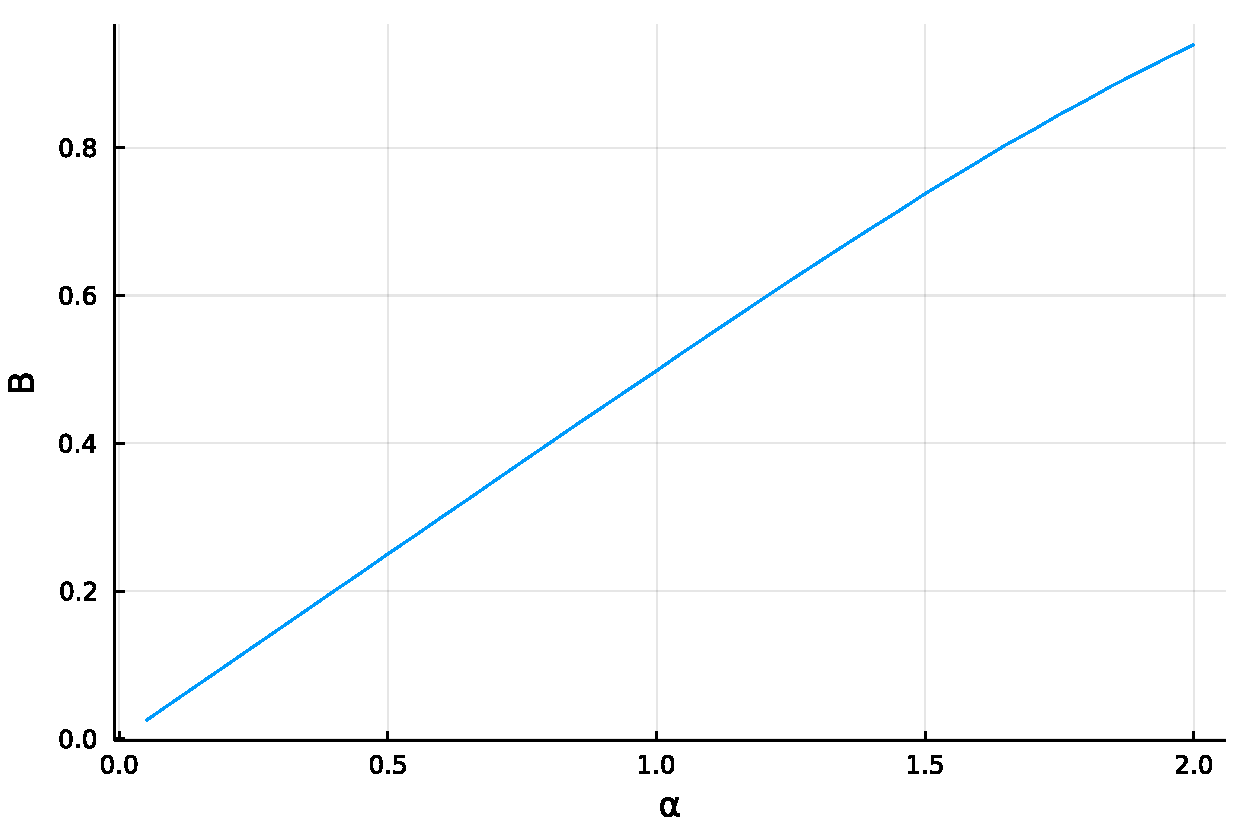
\includegraphics[width=\textwidth]{fig/plot/A_B.pdf}
		\caption{Zależność $B$ od $\alpha$ w równaniu $f(x)=A\left[x(1-x)\right]^B$.}
		\label{eq:A_B}
	\end{figure}
	Ponieważ w skrajnych punktach, czyli dla $x=0$ oraz $x=1$ czas wyjścia musi być zerowy, a największa wartość jest przyjmowana w połowie przedziału, rozpatrywałem początkowo krzywe w postaci $f(x)=A\left[x(1-x)\right]^B$. Parametry $A$ oraz $B$ zostały dopasowane przy pomocy pakietów matematycznych. Na rysunku \ref{eq:A_B} widać liniową zależność $B=\alpha/2$. 
%	\begin{wrapfigure}{l}{0.45\textwidth}
%		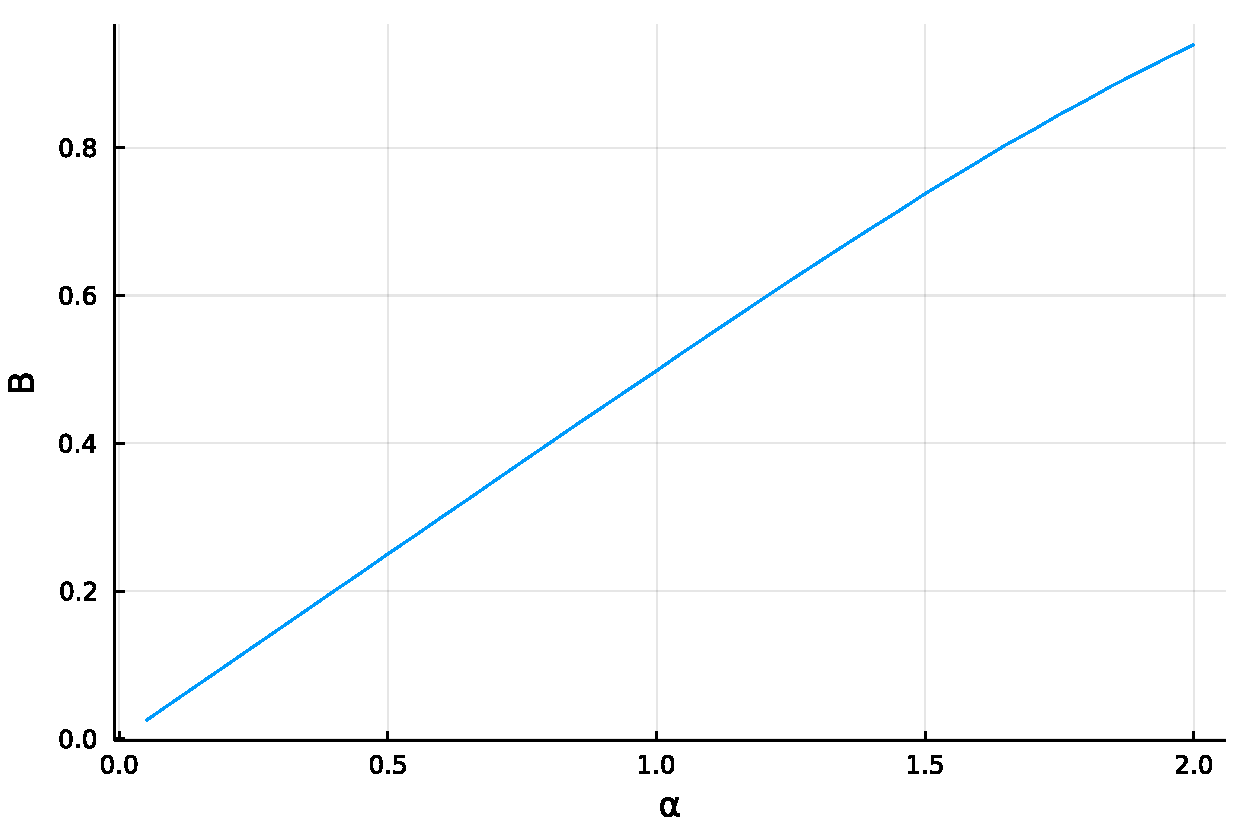
\includegraphics[width=0.43\textwidth]{fig/plot/A_B.pdf}
%		\caption{Zależność $B$ od $\alpha$ w równaniu $f(x)=A\left[x(1-x)\right]^B$.}
%		\label{eq:A_B}
%	\end{wrapfigure}
	\begin{figure}[H]
		\animategraphics[controls,loop,width=\columnwidth]{8}{anim/time/anim}{1}{40}\caption{Animacja czasu wyjścia w zależności od $\alpha$ oraz punktu początkowego.}\label{anim:time}
	\end{figure}
	\noindent Z animacji możemy odczytać, że dopasowana funkcja rzeczywiście dobrze przybliża wygenerowaną krzywą. Dodatkowo dla $\alpha=2$ otrzymujemy wzór, który otrzymaliśmy w naszym poprzednim raporcie\textsuperscript{\cite{rap}}.
	
	
	\section{Prawdopodobieństwo wyjścia przez dany koniec}
	\noindent Dodatkowo oszacowaliśmy prawdopodobieństwo wyjścia przez dany z końców. Z symetrii procesu, wystarczy wyznaczyć prawdopodobieństwo wyjścia przez jeden z końców. W naszym przypadku obliczamy prawdopodobieństwo
	\begin{equation}\label{eq:out}
		\mathbb{P}\left(X^y_{\widetilde\tau^y}=1\right).
	\end{equation}
	Do oszacowania ponownie skorzystaliśmy z metody Monte Carlo. Z powodu dyskretyzacji generowanej trajektorii, musieliśmy przekształcić wzór \eqref{eq:out} do postaci
	\begin{equation}
		\mathbb{P}\left(X^y_{\widetilde\tau^y}\geq1\right).
	\end{equation}
	Podobnie, jak w przypadku szukania wartości oczekiwanej, wynik ten będzie zależał od wartości $\alpha$. Dlatego wynik symulacji przedstawiliśmy w postaci animacji.
	\begin{figure}[H]
		\animategraphics[controls,loop,width=\columnwidth]{8}{anim/out/anim}{1}{40}\caption{Animacja prawdopodobieństwa wyjścia przez dany koniec w zależności od $\alpha$ oraz punktu początkowego. Legenda przedstawia równanie krzywych, gdzie, dla czytelności, zastosowano notację $(y-0.5)^a=\text{sign}(y-0.5)\cdot|y-0.5|^a$.}\label{anim:out}
	\end{figure}
	\noindent Co ciekawe, z animacji możemy odczytać, że dla małych wartości $\alpha$, prawdopodobieństwo wyjścia przez dany koniec w małym stopniu zależy od punktu startowego $y$. Dopasowanie krzywej, do wygenerowanych danych, nie było już tak proste, jak w poprzednich przypadkach. Na animacji \ref{anim:out} zostały dopasowane dwie krzywe do wykresów. Czerwona krzywa (równanie postaci $A\tan\left(\frac{\pi}{2}\left(x-0.5\right)^B\right)+0.5$) lepiej przybliża wynik symulacji dla nie dużych ($<1.3$) wartości $\alpha$. Natomiast z pozostałymi wartościami lepiej sobie radzie krzywa zielona (równanie postaci $A\left(x-0.5\right)^B+1/2$), która dla $\alpha=2$ przyjmuje taką samą postać, jaką otrzymaliśmy w poprzednim raporcie\textsuperscript{\cite{rap}}. Dodatkowo porównując wartości $\alpha$ z $B$ otrzymujemy poniższy wykres.
	\begin{figure}[H]
		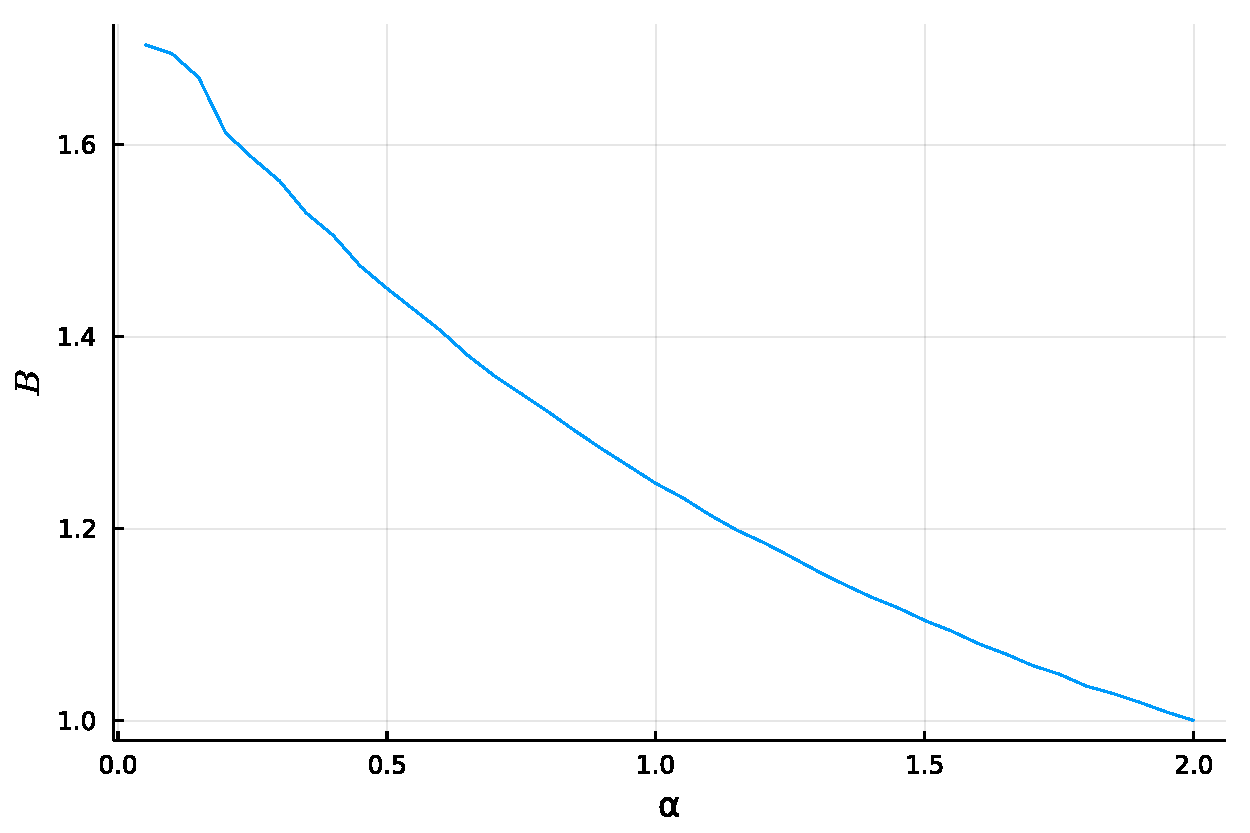
\includegraphics[width=\columnwidth]{fig/plot/A_B_out.pdf}\caption{Zależność $B$ od $\alpha$ w równaniu $f(x)=A\left(x-0.5\right)^B+0.5$.}
	\end{figure}



%	
%	\section{Podsumowanie}
%	\noindent W zadaniu 1, korzystając z różnych metod statystycznych, udało nam się dopasować model klasycznego procesu Ryzyka do danych, co potwierdziło między innymi porównanie funkcji średniej procesu ze średnią z trajektorii z danych. Następnie wykorzystaliśmy wyznaczony model do oszacowania prawdopodobieństwa ruiny. Dokonaliśmy tego korzystając z metody Monte Carlo, a w przypadku nieskończonego czasu, ogromnie przydatny okazał się wzór Pollaczka-Chinczyna. Zgodnie z intuicją okazało się, że wraz ze zwiększaniem czasu, prawdopodobieństwo ruiny rośnie, jednak nie może przekroczyć tego dla nieskończonego czasu.\vspace{1.5mm}\\
%	\noindent Celem drugiego zadania było oszacowanie dwóch funkcji.
%	Zanim do tego przystąpiliśmy, pokazaliśmy, że rozpatrywany przedział mogliśmy wybrać swobodnie. W prosty sposób można uogólnić otrzymane wyniki na dowolny inny przedział. Obie funkcje oszacowaliśmy metodą Monte Carlo. W ten sposób otrzymaliśmy szukane funkcje
%	\begin{equation*}
%		\mathbb{E}\tau^x=-(x-b)(x-a)\quad\text{ oraz }\quad\mathbb{P}\left(B^x_{\tau^x}=b\right)=\frac{x-a}{b-a}.
%	\end{equation*}
%	Otrzymane wyniki bardzo dobrze odzwierciedlają wartości teoretyczne.\vspace{1.5mm}\\
%	\noindent Dodatkowo podczas symulacji zauważyliśmy, jak ważne jest generowanie procesu Wienera z odpowiednio małym krokiem czasowym. Wraz ze wzrostem wielkości kroku, rósł średni czas wyjścia procesu. By uzyskać dokładne dane, generowaliśmy proces z krokiem $h=10^{-4}$.
%	
%	

	\section{Podsumowanie}
	\noindent Udało nam się dopasować funkcję do szukanej wartości oczekiwane. Po uwzględnieniu zależności \eqref{eq:tau_przeskalowane} otrzymaliśmy wynik
	\begin{equation}
		\mathbb{E}\tau^x=A\left(b-a\right)^\alpha\left[y(1-y)\right]^{(\alpha/2)},
	\end{equation}
	gdzie $y=(x-a)/(b-a)$ oraz $A\in[1, 1.5]$ jest wartością zależną od $\alpha$. Oszacowaliśmy jeszcze prawdopodobieństwo wyjścia przez dany koniec przedziału. Wynik może wydawać się lekko zaskakujący, gdyż dla małych wartości $\alpha$, zależy on w niewielki stopniu od punktu początkowego procesu.
	
	\newpage
	\begin{thebibliography}{1}
		\bibitem{Levy_def}
		\url{https://people.bath.ac.uk/ak257/LCSB/part1.pdf}
		\bibitem{art}
		\url{http://prac.im.pwr.edu.pl/~hugo/publ/SFB2005-008_Borak_Haerdle_Weron.pdf}
		\bibitem{rap}
		\url{https://drive.google.com/file/d/1Mutv7S7TcRbvwD8fzdeqaEdPUFSPHPcf/view?usp=sharing}
	\end{thebibliography}


\end{document}